
\chapter{Application}
\label{cha:application}

This chapter present two more involved cases of identification. The first case
is identification of the COST beam, introduced as a standard test case for
polynomial nonlinearities, ie. two polynomial nonlinearities at the same DOF.
The second case demonstrate the usage of cubic spines to identify a system with
two different clearances. The clearance distances are also found.


\section{COST beam}
\label{sec:cost-beam}

The European action COST F3 nonlinear beam \autocite{GOLINVAL2003} was
introduced in 2003 as a benchmark system for nonlinear vibrations. The
experimental setup is shown in fig. \ref{fig:beam_setup} and consists of a
clamped beam with a thin beam part at the end of the main beam.

\begin{figure}[!ht]
  \centering
  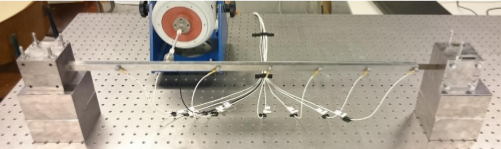
\includegraphics[width=1\textwidth]{nlbeam/beam_setup.png}
  \caption{Experimental setup for the COST beam. Both vertical and horizontal
    setups were tested. Horizontal setups avoids gravitational effects which
    cannot be ignored due to the thin beam.}
  \label{fig:beam_setup}
\end{figure}


Accelerations are measured evenly along the beam at seven locations and excited
at node two.
From \textcite{lenaerts2003a} is it known that the system exhibit a (geometric)
cubic nonlinearity located at the tip of the main beam. Using data given at the
Nolinsys course, the beam will be identified as an example of a multiple inputs,
multiple outputs(MIMO) system. After successful identification a FE model is
built using the identified parameters and used for further examination.

The cubic nonlinearity is described to be due to \textit{large deformation of the
  tip of the thin beam}. This is a bit vague description and could include both
large rotations and midplane stretching. As both ends are clamped, the
nonlinearity probably stems from midplane stretching of the thin beam.
In \autocite{juel2003a} it is shown how both midplane stretching and large
rotations of a beam leads to a duffing equation with a cubic hardening.

Due to the thin beam, the effect of gravity is not negligible. In a vertical
setup the static deflection at the beam tip imposes a non-negligible prestress
in the thin beam, giving a nonsymmetric restoring force. This is identified as a
quadratic nonlinearity and the effect is simply removed by using a horizontal
setup.

\subsection{Identification}

The time series were obtained from University Liege(ULg), where the beam was
built as part of the COST F3 project. Unfortunately, despite several request,
only noise-free simulated data were given.

For characterisation the beam is excited with a sine sweep. The wavelet
transform and RFS is seen in fig. \ref{fig:nlbeam_characterisation}. From the
WT, the fundamental forcing frequency is seen along with even(2:1,4:1,...) and
uneven(3:1,5:1,...) higher harmonics. These higher harmonics are symptoms of
quadratic and cubic nonlinearities.
As the FRF shows the total restoring force, it is hard to identify the correct
nonlinear function. However the asymmetry indicate an even nonlinearity and the general
shape resembles a cubic polynomial.

\begin{figure}
  \centering
  \begin{subfigure}[b]{0.45\textwidth}
    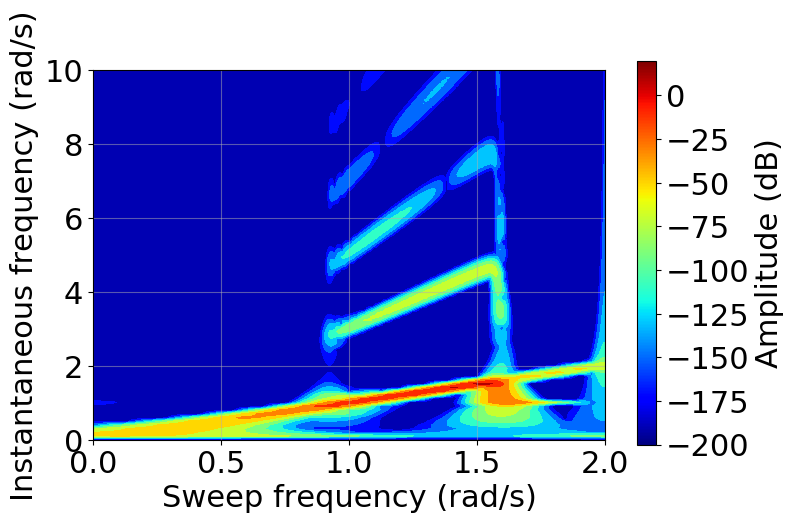
\includegraphics[width=\linewidth, height=6cm]{nlbeam/wt.png}
    \caption{}
  \end{subfigure}
  ~
  \begin{subfigure}[b]{0.45\textwidth}
    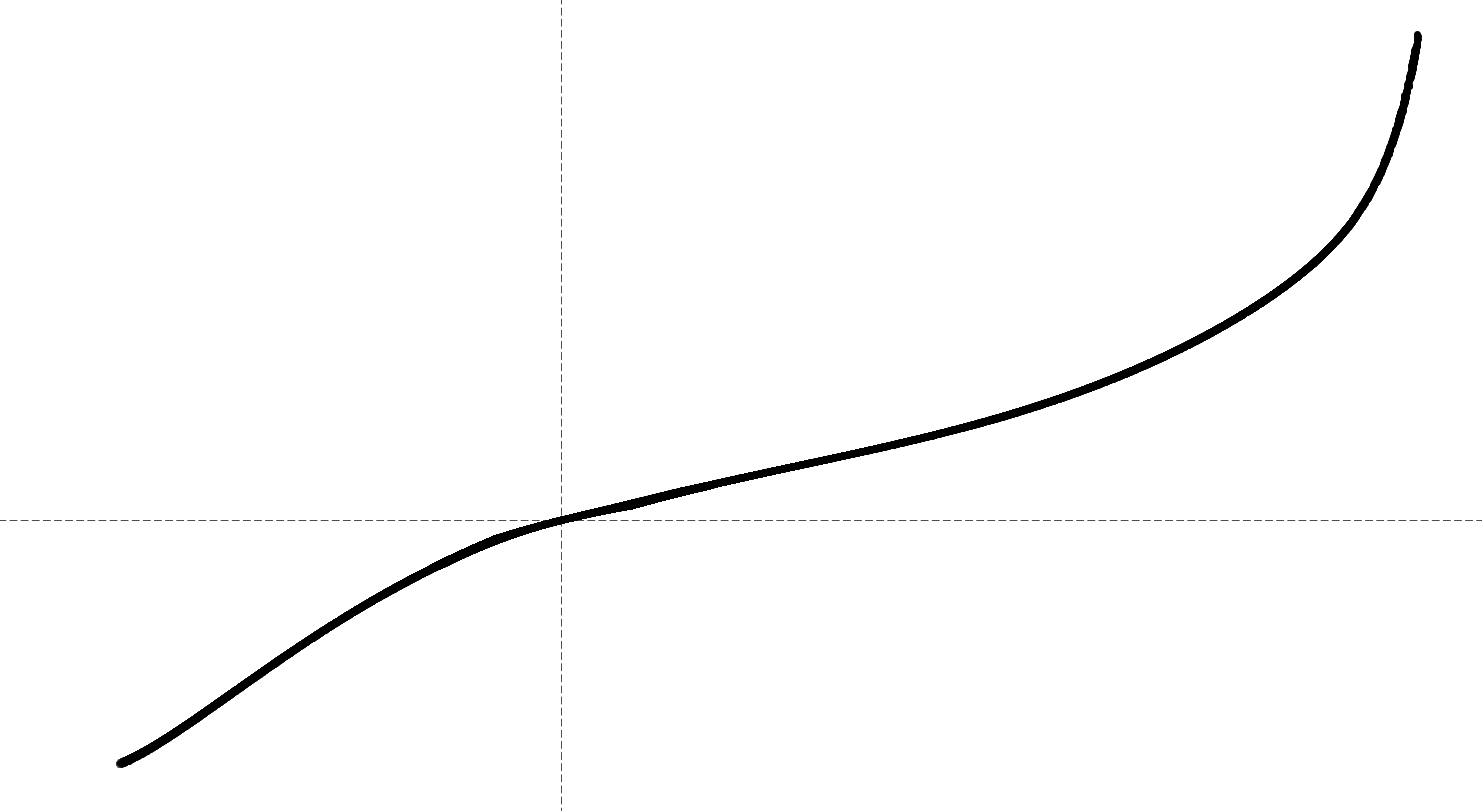
\includegraphics[width=\linewidth, height=6cm]{nlbeam/rfs.tikz}
    \caption{}
  \end{subfigure}
  \caption{Characterisation using a forward sine sweep. Sweep rate: 10Hz/min.
    Shown for the tip of the main beam.
    \textbf{(a)}: Wavelet transform;
    \textbf{(b)}: Restoring force surface showing the restoring force.}
  \label{fig:nlbeam_characterisation}
\end{figure}


For estimation the beam is excited with a periodic broadband input with flat
amplitude spectrum, i.e. a multisine at low and high level. At low and high
level, the beam behaves linear and nonlinear respectively. To avoid leakage in
the identification due to transient behavior, the periods used are selected from
a plot of the periodicity. From fig. \ref{fig:nlbeam_per} is seen that
transients are apparent in the first two periods and not apparent in periods
4-7, which are used for the identification.

\begin{figure}[!ht]
  \centering
  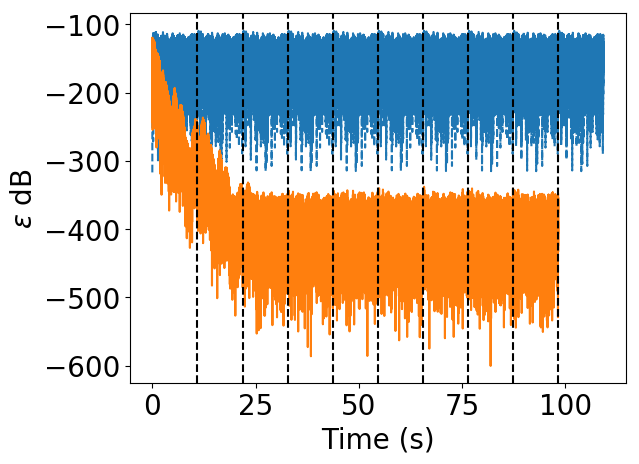
\includegraphics[width=0.6\textwidth]{nlbeam/fnsi/per.png}
  \caption{Periodicity of recorded signal at high level wrt. the last period.
    Measured at the nonlinear dof. Low level excitation is not shown, as it is
    not used for NL estimation.}
  \label{fig:nlbeam_per}
\end{figure}

Figure \ref{fig:nlbeam_stab} shows the stabilisation diagram used for determine
model order. Fig. \ref{fig:nlbeam_stab}(a) is used for linear identification and
is fully stabilised at order 6. Fig. \ref{fig:nlbeam_stab}(b) shows the
nonlinear system identified with linear analysis, ie. without specifying
nonlinear basis functions. The first mode does not stabilise, which normally
indicates that the supplied basis functions are inadequate to represent the
nonlinearity. Fig. \ref{fig:nlbeam_stab}(c) shows the stabilisation after
using a quadratic and cubic basis function. The first mode stabilises at
model order 6, ie. the identification is most likely trustworthy and the
nonlinearities are described by these functions.

\begin{figure}
  \centering
  \begin{subfigure}[b]{0.45\textwidth}
    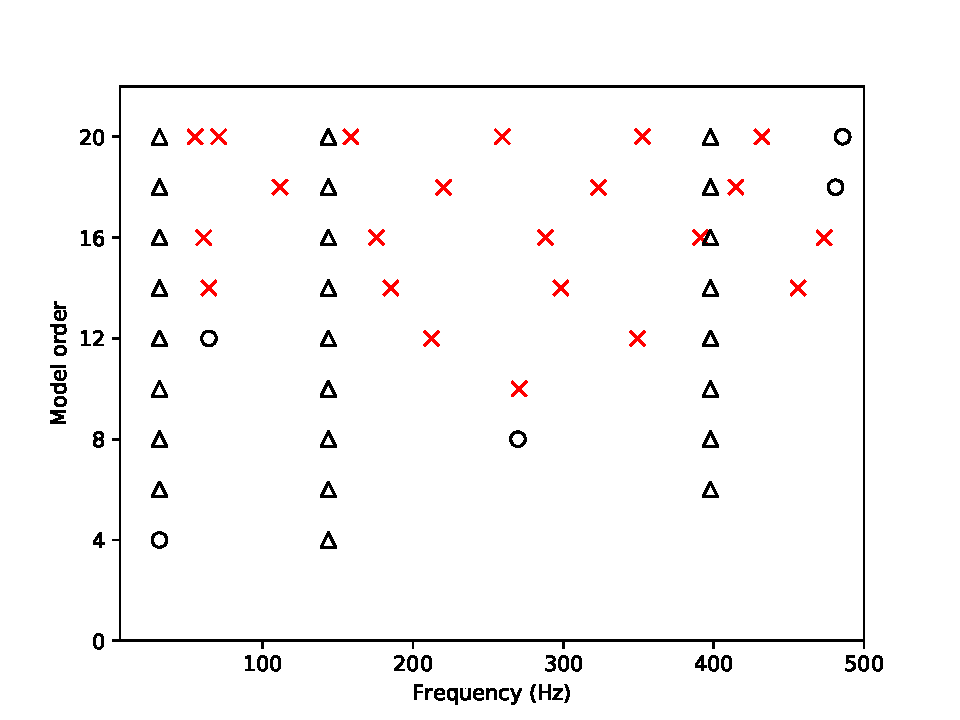
\includegraphics[width=\linewidth, height=6cm]{nlbeam/fnsi/stab_lin}
    \caption{}
  \end{subfigure}
  ~
  \begin{subfigure}[b]{0.45\textwidth}
    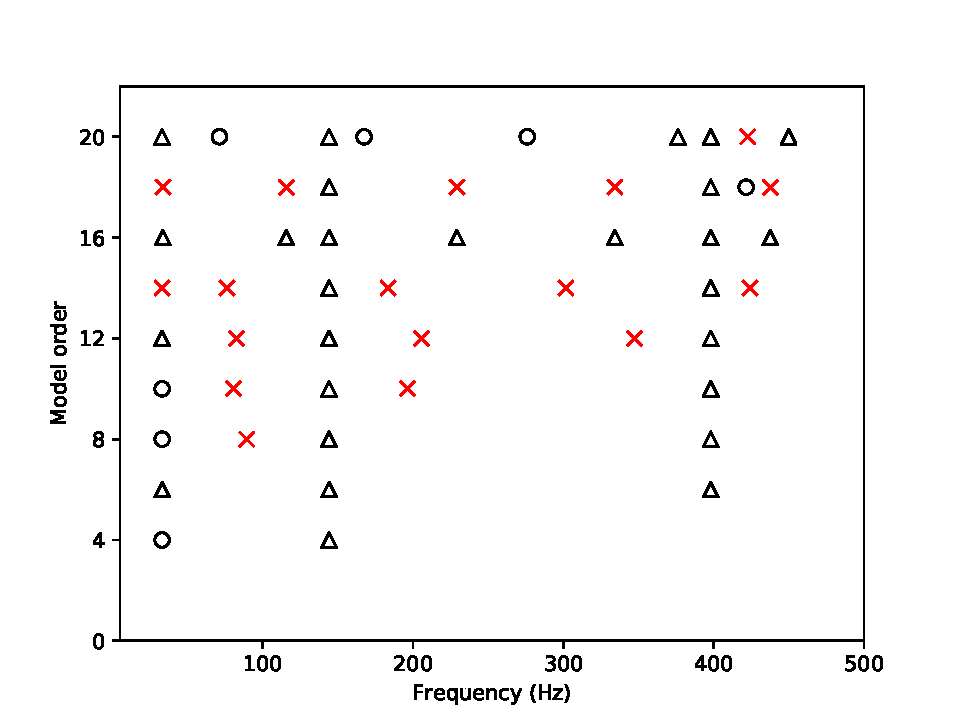
\includegraphics[width=\linewidth, height=6cm]{nlbeam/fnsi/stab_nlin1}
    \caption{}
  \end{subfigure}
  \\
  \begin{subfigure}[b]{0.45\textwidth}
    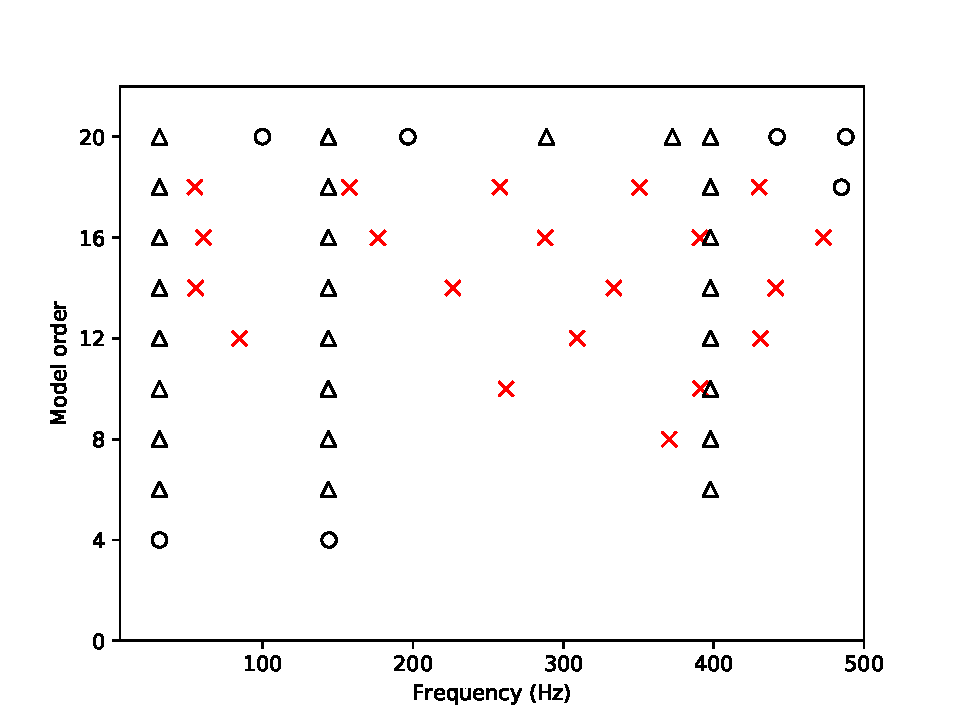
\includegraphics[width=\linewidth, height=6cm]{nlbeam/fnsi/stab_nlin2}
    \caption{}
  \end{subfigure}
  \caption{Estimation of model order.
    \textcolor{red}{$\pmb\times$}: new frequency(pole);
    $\pmb\circ$: extra stabilisation in MACX;
    $\pmb\triangle$: full stabilisation.
    \textbf{(a)}: Low level, linear identification;
    \textbf{(b)}: High level, linear identification - no stabilisation of first mode;
    \textbf{(c)}: High level, nonlinear identification - stabilisation of first mode;
  }
  \label{fig:nlbeam_stab}
\end{figure}

The identified linear parameters are shown in table \ref{tab:nlbeam_par}. At
high excitation using linear analysis, the natural frequency increases for the
first mode which is expected from a hardening nonlinearity.
Using the two basis functions, ie. nonlinear analysis, the parameters are
estimated to be same as obtained at low level, ie. correct.

\begin{center}
  \begin{tabular}{@{} c *{4}{c} @{}}
    \hline
    & Mode & Frequency (Hz) & Damping ration (\%) & Deviation from linear freq. (\%) \\
    \hline
    %\cmidrule{1-3}
    &1 & 31.3 & 1.27 \\
    &2 & 143.6 & 0.29 \\
    \rot{\rlap{~Low}}
    &3 & 397.8 & 0.14 \\
    \hline
    &1 & 33.1 & 1.08 & 5.7 \\
    &2 & 144.1 & 0.29 & 0.3 \\
    \rot{\rlap{High}}
    &3 & 398.0 & 0.14 & 0.05 \\
    \hline
    &1 & 31.3 & 1.27 & $10^{-3}$ \\
    &2 & 143.6 & 0.29 & $10^{-5}$ \\
    \rot{\rlap{~High}}
    &3 & 397.8 & 0.14 & $10^{-6}$ \\
    \hline
  \end{tabular}
  \captionof{table}{Estimated linear natural frequencies and damping ratios for
    the COST beam.
    \textbf{(upper)}: Low level, linear identification;
    \textbf{(middle)}: High level, linear identification;
    \textbf{(lower)}: High level, nonlinear identification.
  }
  \label{tab:nlbeam_par}
\end{center}

The identified nonlinear coefficients are shown in figure \ref{fig:nlbeam_knl}.
The deviation of the real part is just within 1\% and the imaginary part are
around three orders of magnitude smaller, indicating a good identification.

\begin{figure}[!ht]
  \centering
  \begin{subfigure}[b]{0.45\textwidth}
    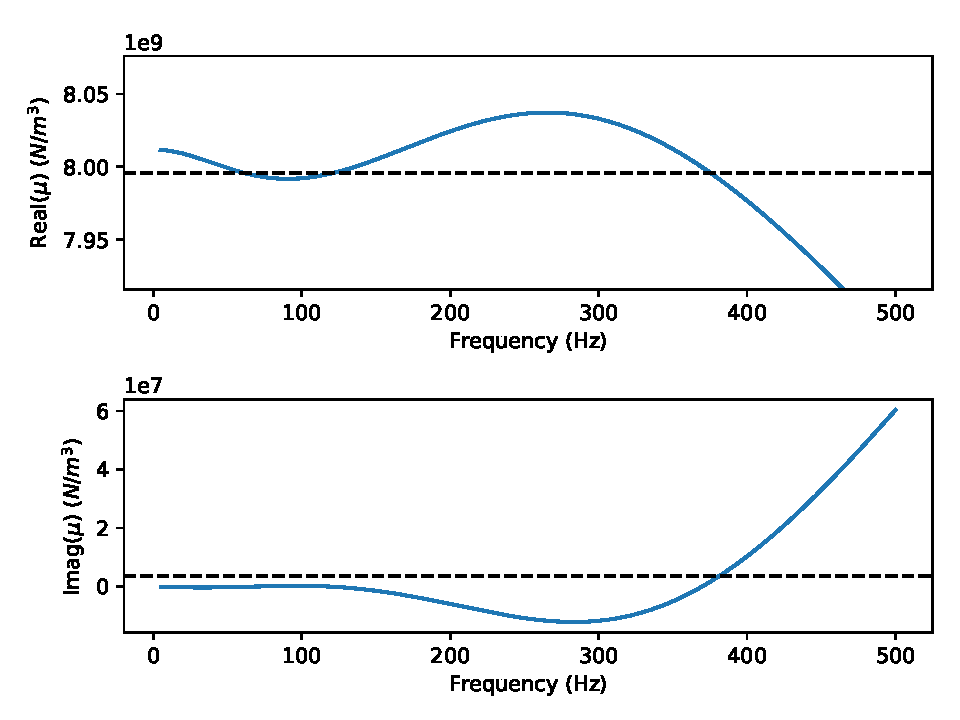
\includegraphics[width=\linewidth]{nlbeam/fnsi/knl0.pdf}
    \caption{}
  \end{subfigure}
  ~
  \begin{subfigure}[b]{0.45\textwidth}
    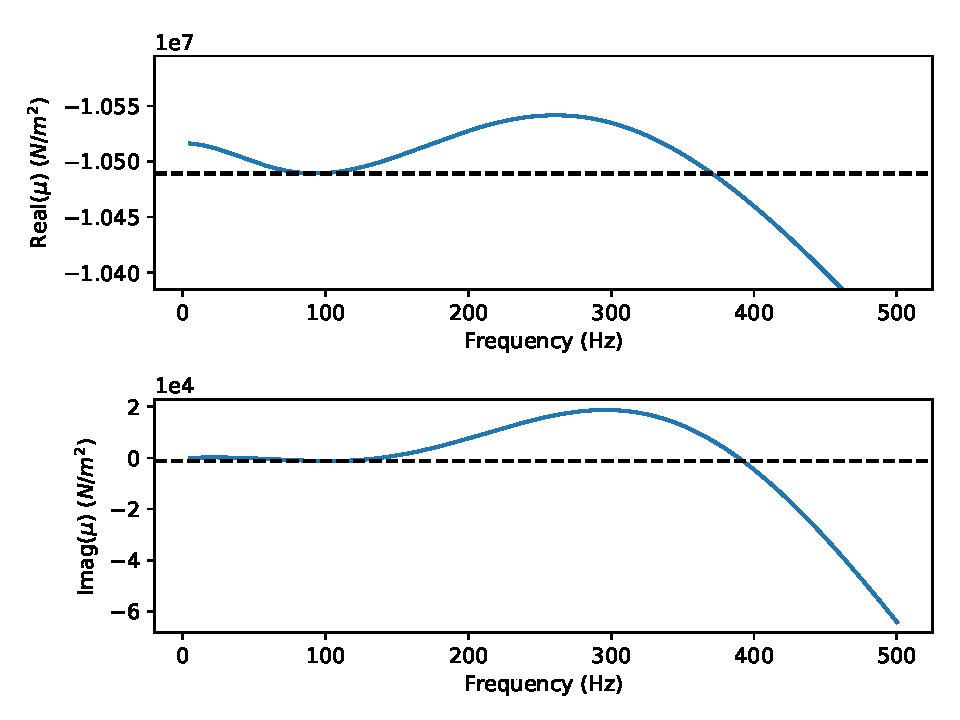
\includegraphics[width=\linewidth]{nlbeam/fnsi/knl1.pdf}
    \caption{}
  \end{subfigure}
  \caption{Real and imaginary part of estimated nonlinear coefficients $\mu_1$
    and $\mu_2$. The variation of Re($\mu$) is seen to be within a 1 interval.
    The imaginary part is about three orders of magnitude smaller. Both
    indicates a good quality of the estimation. The spectral averages of the
    real part and logarithmic ratio between the real and imaginary part
    ($\log_{10} \left(\frac{\Re(\mu)}{\Im(\mu)} \right)$) are:
    \textbf{(a)}: $\mu_1 = 8.0 \times 10^9 m/n^3$, ratio = 3.34;
    \textbf{(b)}: $\mu_2 = -1.05 \times 10^7 m/n^2$, ratio = 3.96.
  }
  \label{fig:nlbeam_knl}
\end{figure}


Finally fig. \ref{fig:nlbeam_frf} shows the FRF. Nonlinear distortion is seen
from the signal at high level excitation. The FRF(blue) from low level excitation and
identified by FNSI with basis functions(green) match.

\begin{figure}[!ht]
  \centering
  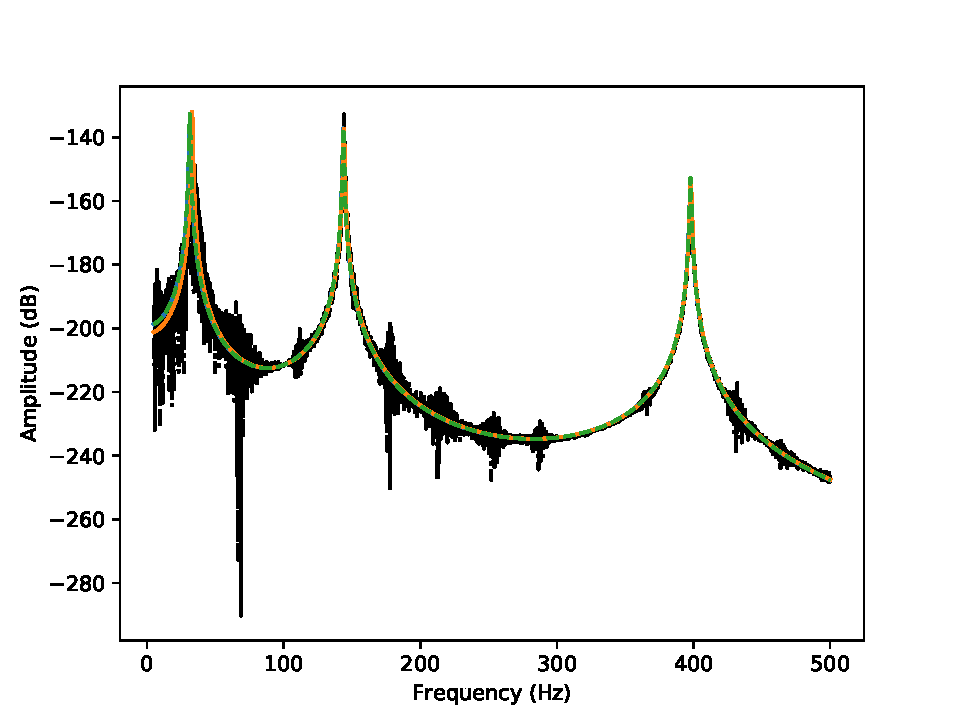
\includegraphics[width=0.7\textwidth, height=8cm]{nlbeam/fnsi/frf.pdf}
  \caption{FRF. Nonparametric(NP) is FRF directly from signal, parametric is
    identified FRF.
    \sampleline{}: NP from high level excitation;
    \textcolor{blue}{\sampleline{}}: NP from low level excitation.
    \textcolor{orange}{\sampleline{}}: Linear parametric from high level excitation.
    \textcolor{green}{\sampleline{dashed}}: nonlinear parametric from high level excitation.
}
  \label{fig:nlbeam_frf}
\end{figure}

\subsection{Design}

The test setup is modelled as a FE model shown in fig \ref{fig:nlbeam_fem},
using 14 and 3 two-dimensional Bernoulli-Euler beam elements for the main and
thin beam respectively. The connection between the two beams is modelled by an
additional linear rotational stiffness, as suggested in
\autocite{lenaerts2003a}, resulting in a model with 35 dofs.
% In traditional FEM, boundary conditions can be enforced
% in different ways; either modifying the stiffness matrix or the load vector.
% With the methods presented here, boundary conditions should always be enforced
% by modifying the stiffness matrix, i.e. for fixed dofs all rows and columns
% relating to these dofs are removed, which is why the system ends up having 35
% dofs.

\begin{figure}[!ht]
  \centering
  \def\svgwidth{10cm}
  \import{fig/nlbeam/}{beam_fem.pdf_tex}
  \caption{FE model of the COST beam.}
  \label{fig:nlbeam_fem}
\end{figure}

The geometric properties are also given in \autocite{lenaerts2003a} and listed
together with the mechanical properties in tables \ref{table:nlbeam_prop}.
\begin{center}
  \resizebox{\columnwidth}{!}{%
 \begin{tabular}{l*{4}{c}}
  %\begin{tabular}{p{3.1cm}p{2cm}*{3}{c}}
    \hline
  & Length(m) & Width (m) & Thickness (m) \\
  \hline
  Main beam & 0.7 & 0.014 & 0.014 \\
    Thin beam & 0.04 & 0.014 & 0.0005 \\
    \\
  \hline
  Young's modulus\newline (N/$m^2$) & Density\newline (kg/$m^3$) & $\mu_1$ (N/$m^3$) & $\mu_2$ (N/$m^2$) & Damping  \\
  \hline
  $2.05\times 10^{11}$ & 7800 & $8\times 10^{9}$ & $-1.05\times 10^{7}$ &  $\bm C = 3 \times 10^{-7} \bm K + 5\bm M$ \\
  \hline
 \end{tabular}
 }
\captionof{table}{Geometric and mechanical properties for the nonlinear beam}
\label{table:nlbeam_prop}
\end{center}


The damping is proportional damping, giving a modal damping ration of $1.27\%$
for the first linear mode which is high for a steel beam. But large
displacements tends to be higher damped, thus the damping is not expected to be
same for the linear and nonlinear case.

Figure \ref{fig:nlbeam_sweep} shows a comparison between a linear forward and
backward sine sweep and the NFRC computed by HB. The response
is asymmetric due to the presence of the quadratic nonlinearity. The jump down
occurs because of the hardening(cubic) behavior.

\begin{figure}[!ht]
  \centering
  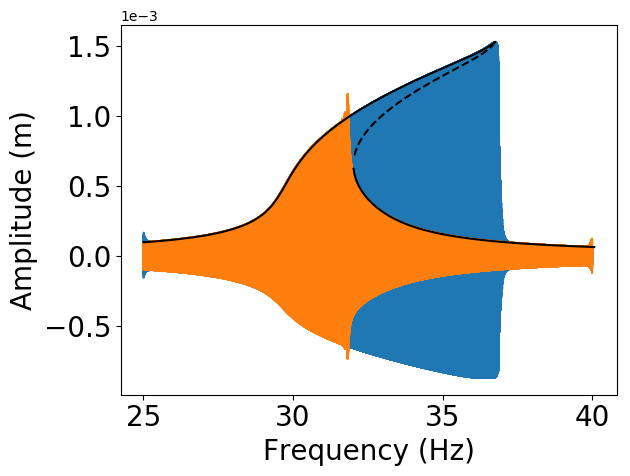
\includegraphics[width=0.7\textwidth]{nlbeam/hb/sweep.png}
  \caption{Comparison between forward and backward sine sweep(colours) with
    HB(black line).
    Sweep parameters: Amplitude: 3N, sweep rate: 10Hz/min. Stability is indicated for
    HB. Shown for the tip of the main beam, ie. the nonlinear connection.}
  \label{fig:nlbeam_sweep}
\end{figure}

Figure \ref{fig:nlbeam_hb_components} shows the evolution of the harmonic
components along the curve. As expected from the asymmetry, there is strong
participation of the constant term, followed by the 2nd harmonic. Both due to
the quadratic nonlinearity.

\begin{figure}[!ht]
  \centering
  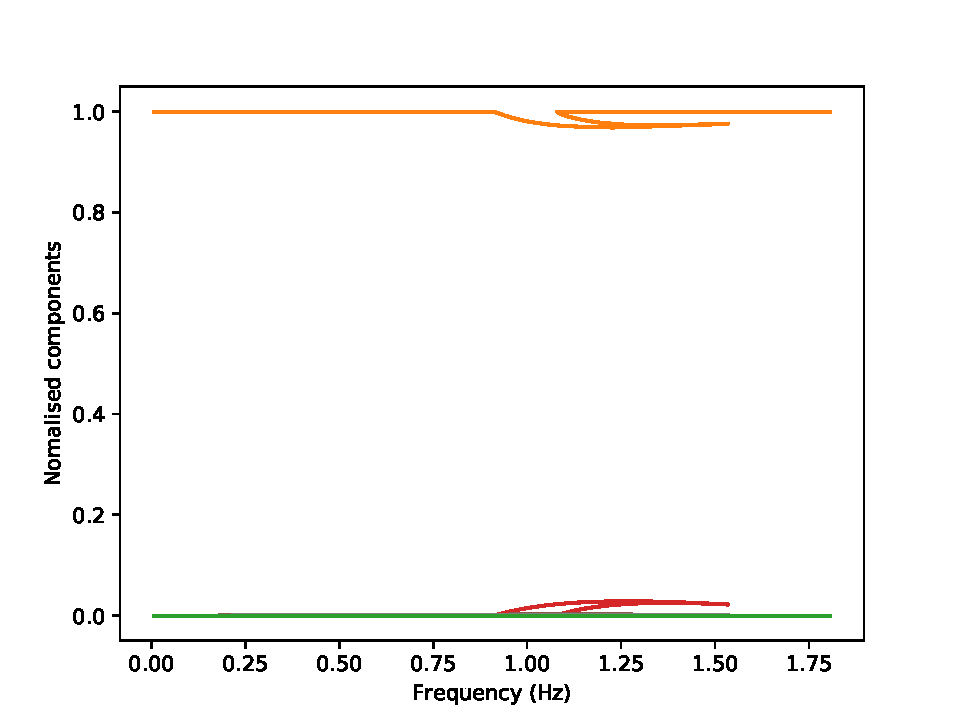
\includegraphics[height=6cm,width=0.7\textwidth]{nlbeam/hb/har}
  \caption{Evolution of HB components.
    \textcolor{blue}{\sampleline{}}: Constant;
    \sampleline{}: 1st;
    \textcolor{orange}{\sampleline{dotted}}: 2nd;
    \textcolor{green}{\sampleline{dash pattern=on .7em off .2em on .2em off .2em}}: 3th;
    \textcolor{red}{\sampleline{}}: 4th;
    \textcolor{purple}{\sampleline{dashed}}: 5th;
  }
  \label{fig:nlbeam_hb_components}
\end{figure}

The NNMs of the underlying conservative system is shown in fig
\ref{fig:nlbeam_nnm}. The NNM frequency increases with increasing energy, which
is due to the hardening behavior of the nonlinear stiffness. The inserts shows
the modal shapes of the main beam for different energy levels. The modal shapes
are synchronous.
The FEPs shows one branch emerging from each NNM backbone. These are called
tongues and are said to reveal internal resonance. The tongue for the first NNM,
fig. \ref{fig:nlbeam_nnm}(a), shows a 9:1 internal resonance between the first
and third NNM. Their linear frequencies are incommensurate as seen in table
\ref{tab:nlbeam_par}, but the frequency for the first NNM increases more rapidly
than for the third NNM, resulting in a 9:1 ratio between the frequencies is
realised. This might be of more theoretical interest, as a high energy level
indicate very large displacements.

\begin{figure}[!ht]
  \centering
 \begin{subfigure}[b]{0.45\textwidth}
    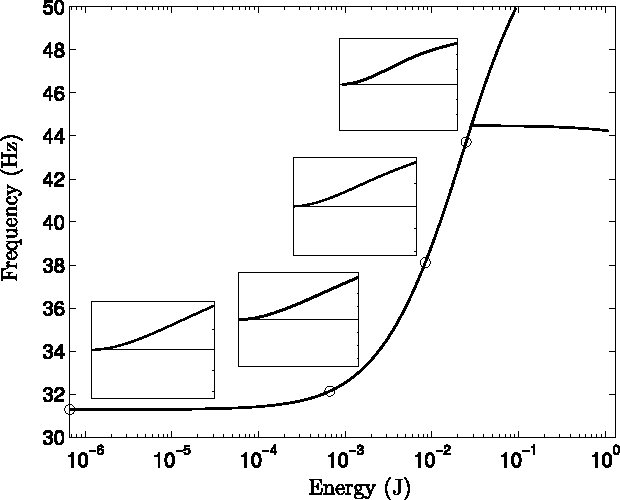
\includegraphics[width=\linewidth]{nlbeam/nnm/nnm1.pdf}
    \caption{}
  \end{subfigure}
  ~
  \begin{subfigure}[b]{0.45\textwidth}
    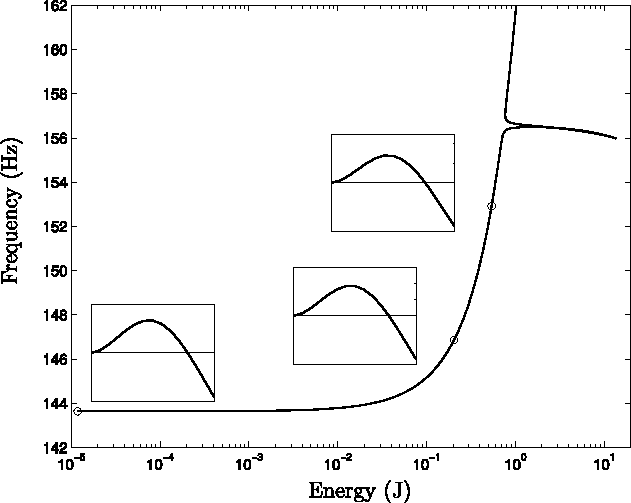
\includegraphics[width=\linewidth]{nlbeam/nnm/nnm2.pdf}
    \caption{}
  \end{subfigure}
  \caption{Frequency-energy plot(FEP) of the
    \textbf{(a)} first- and
    \textbf{(b)} second NNM. Inserts show the NNM shapes (displacements of the
    main beam) for different energy levels.}
  \label{fig:nlbeam_nnm}
\end{figure}

Finally, the NNM backbone traces the lotus as seen in fig.
\ref{fig:nlbeam_sweep}.

\begin{figure}[!ht]
  \centering
  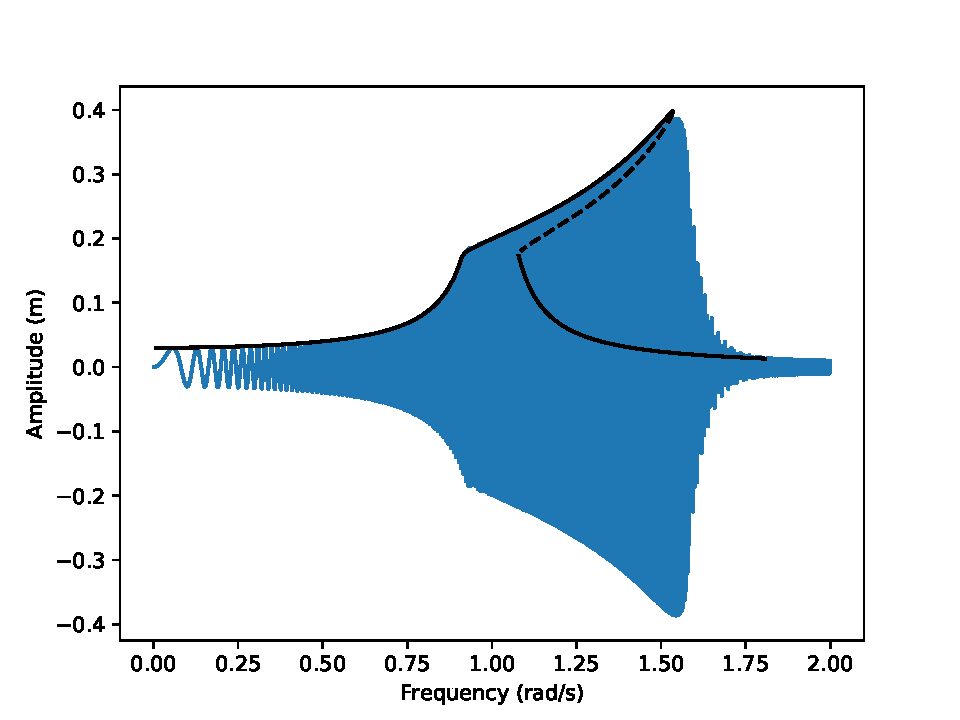
\includegraphics[width=1\textwidth]{nlbeam/hb/nfrc.pdf}
  \caption{
    \textbf{(left)}:
    NFRC for forcing amplitudes (1,2,3,4)N from HB. The dashed line is
    the backbone of the first NNM and tracks the lotus;
    \textbf{(right)}:
    Phase lag wrt. the excitation force.;
    Shown for the tip of the main beam. $\square$
    denote $F=4N$.
    }
  \label{fig:nlbeam_sweep}
\end{figure}


\FloatBarrier
\section{System with clearences}
\label{sec:syst-with-clear}

A single DOF model with two clearances is simulated to obtain data for
characterisation with WT and RFS and identification with FNSI.

\subsection{Model}

The model is a clamped-free beam with a pair of elastic stops at the free end
with asymmetrical clearance distances $a_\pm$, see fig
\ref{fig:clear_schematic}.


\begin{figure}[!ht]
  \centering
  \centering
  \def\svgwidth{10cm}
  \import{fig/contact/}{beam.pdf_tex}
  \caption{Beam with elastic stops}
  \label{fig:clear_schematic}
\end{figure}


The bending vibrations of the beam is given by
\begin{equation}
  \label{eq:clear_EOM}
  \rho A \frac{\p^2 u(z,t)}{\p t^2} + \frac{\p^2}{\p z^2}
  \left( EI \frac{\p^2 u(z,t)}{\p z^2}  \right) +
  f_{res}(u(z_b,t)) \delta (z-z_b) +
  P_0 \sin(\Omega t) \delta(z-z_f)= 0
\end{equation}
where $EI, \rho, A, \delta(z), Q_0, u(z,t)$ denotes the stiffness bending, mass
density, cross section area, Dirac delta function, forcing amplitude and
relative transverse displacement, respectively, for the assumed uniform beam.
The external force act in $z_f$. The vibro-impact force at the impact location
$z_b$ is given by

\begin{equation}
  \label{eq:clear_vibro_force}
  f_{res}(u) =
  \begin{cases}
    k_+(u - a_+) & u \geq a_+ \\
    0 &  a_+ > u > a_- \\
    k_-(u - a_+) & u \leq - a_- \\
  \end{cases}
\end{equation}
where $a_\pm$ are the clearance distances and $k_\pm$ the associated
stiffness's. Thus the stops behaves as one-sided springs.

The left end is clamped, giving the boundary conditions
\begin{equation}
  u(0,t) = 0, \quad u(0,t)_z = 0
\end{equation}
and at the right end, between stops, the beam moves freely giving a free moment
and transverse stress condition
\begin{equation}
 a_+ > u > a_-: \quad u_{zz}(L,t) = 0, \quad u_{zzz}(L,t) = 0
\end{equation}

When the elastic stops are hit, the stress $\sigma = k^2u_{zzz}$ is no longer
zero
\begin{equation}
  a_+ < u, u < a_-: \quad \sigma(L,t) = - f_{res}(u)
\end{equation}
where $k^2$ is the scaled elastic modulus. Notice that the stress is opposite in
direction to the displacement. For $k_\pm \to \infty$, the stops are rigid and
velocity changes sign instantly at each impact, known as the Signorini
nonpenetration condition.


An approximate solution to \eqref{eq:clear_EOM} is given by the modal expansion
\begin{equation}
  \label{eq:clear_modal}
  u_n(z,t) = \sum_{i=1}^n \phi_i(z) q_i(t)
\end{equation}
where $\phi_i$ is the mode shape related to the $i$'th natural frequency
$\omega_i$; together they define the $i$'th mode for linear system of eq.
\eqref{eq:clear_EOM}, ie. with $f_{res}(u) = 0$.

The modal components $q_i(t)$ satifies the coupled nonlinear differential
equation
\begin{equation}
  \ddot q_i(t) + 2 \xi \omega_i \dot q_i(t) + \omega_i^2 q_i(t) +
  \frac{\phi_i(z_b)}{\rho A L} f_{res}(u_n(z_b,t)) +
  \frac{\phi_i(z_f) Q_0}{\rho A L}\sin(\Omega t)
  = 0, \quad
  \text{for} i=1,...,n
\label{eq:clear_mode_expansion}
\end{equation}
where viscous damping have been added to account for dissipative effects. This
is not easily solved, but a technique to find approximate analytical solutions
to vibro-impact problems is found in \parencite{thomsen2008a}.


\subsubsection{Numerical solution}

By using the approximation eq. \eqref{eq:clear_modal} with
\ref{eq:clear_mode_expansion}, the vector $x(t)= (u(z_1,t),...,u(z_n,t))^T $ is
the solution to the nonlinear FE model eq. \eqref{eq:per_eom}.

To solve the FE model, the derivative of the restoring force must be calculated
and is required to be continuous. This is enforced using local regularisation
with Hermite polynomials in the interval $[a-\Delta, a+\Delta]$, where $2\Delta$
is the size of the regularisation interval.
Figure \ref{fig:fnl_piecewise} shows an example of a regularised tri-linear
restoring force; the purely linear behavior of the restoring force outside the
regularisation interval is kept.

\begin{figure}[!ht]
  \centering
  \def\svgwidth{10cm}
  \import{fig/contact/}{piecewise_linear.pdf_tex}
  \caption{Example of piecewise-linear restoring force. The insert image shows a
    closeup of the effect of the regularization $\Delta$.}
  \label{fig:fnl_piecewise}
\end{figure}


A trilinear model for stiffness' $k_-, k, k_+$ and clearances $a_-, a_+$ is
given by, %\autocite{renson2014_phd}
\begin{equation}
  \label{eq:fnl_piecewise}
  f_{nl}(x) =
  \begin{cases}
    \sign(x) \left( ka_+ + k_+(x-a_+) \right) & x \geq a_+ + \Delta_+ \\
    p_+(t(x)) & a_+ + \Delta_+ > x > a_+ - \Delta_+ \\
    kx & a_+ - \Delta_+ \geq x \geq  -(a_- - \Delta_-) \\
    p_-(t(x)) & -(a_- + \Delta_-) > x > -(a_- + \Delta_-) \\
    \sign(x) \left( ka_- + k_-(x-a_-) \right) & x \leq -(a_- + \Delta_-) \\
  \end{cases}
\end{equation}
where $x$ is the relative distance between the two DOFs defining the nonlinear
connections.

The Hermite polynomials $p_\pm$ are defined as
\begin{equation}
  \label{eq:fnl_herm_pol}
  p_\pm(t) = h_{00}(t)p_k + h_{10}(t)(x_{k+1}-x_k)m_k + h_{01}(t)p_{k+1} + h_{11}(t)(x_{k+1} - x_k)m_{k+1}
\end{equation}
where $p_k$ and $p_{k+1}$ are the values of the restoring force at points $x_k =
\sign(x)(a - \Delta)$ and $x_{k+1} = \sign(x)(a + \Delta)$, respectively. $m_k$
and $m_{k+1}$ are the values of the restoring force derivative at the same $x_k$
and $x_{k+1}$ points; they correspond to the stiffness coefficients k and
$k_\pm$. The local scaled abscissa and $h_{ij}$ functions are

\begin{equation}
  \label{eq:fnl_piecewise_coeff}
  \begin{aligned}
    t(x) &= \frac{x - x_k}{x_{k+1} - x_k}\\
    h_{00}(t) &=  2t^3 - 3t^2 + 1 \\
    h_{10}(t) &= t^3 - 2t^2 + t \\
    h_{01} &= -2t^3 + 3t^2 \\
    h_{11} &= t^3 - t^2 \\
  \end{aligned}
\end{equation}


It should be noted that solving systems with a large difference in stiffness
might not be easy. When the beam hit the stops, some spurious high frequencies
may appear. These spurious frequencies may disappear by choosing a smaller
time-step and if not, the solutions become unstable. In that case a time
integration method with numerical damping should be used. A possibility is to
use a Newmark scheme with $\gamma > \frac{1}{2}$ in order to introduce some
numerical damping in the higher modes. Unfortunately, this scheme is only of
first order and the effect of the damping can affect the lower modes of the
solution and the amplitude of the displacement. Preferable another scheme should
be used, see appendix \ref{sec:newmark_summary}.


\FloatBarrier


%%% Local Variables:
%%% mode: latex
%%% TeX-master: "../report"
%%% End:
